\chapter{Implementation} 
\label{chapter:implementation}
This chapter describes the design of smart contracts and provides the detailed implementation of each function that is adopted in this paper. The smart contract diagram as shown in Figure~\ref{fig:smart_contract_diagram},  all of the organizations have common \(OMgr\) for managing users' information and storing users' status. The ecosystem initiator enables blockchain-based functionality by deploying a \(OMgr\). It offers application binary interface (ABI) files for all participants to easily call smart contract functions.

\begin{figure}[hb]
    \centering
    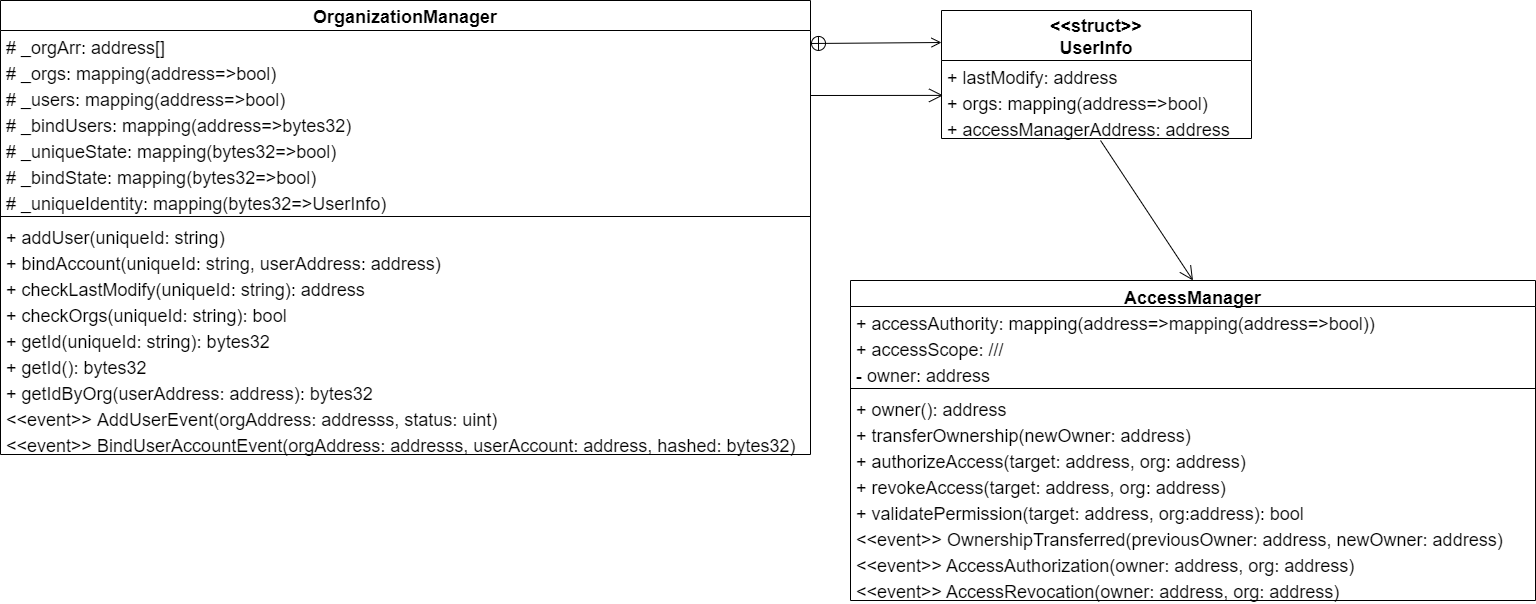
\includegraphics[height=!,width=1\linewidth,keepaspectratio=true]{figures/smart_contract_diagram.png}
    \caption{{\footnotesize Smart Contract Diagram}}
    \label{fig:smart_contract_diagram}
\end{figure}
\section{Smart contract design}
\subsection*{Organization Manager}
The \(OMgr\) is used to manage information that is related to users and organizations, i.e., it records data attributes, users' identity hash value. In Table~\ref{table:userinfo}, the \textit{UserInfo} structure represents an independent \(DI\). After the identity verification process is done as shown in Figure~\ref{fig:identityVerification}, the \(DI\) will be created for users automatically.


\begin{table}[h]
     \centering
     % [] 顯示在 list of tables 的文字
     % {} 顯示在表格上方的文字
     \caption[Table of UserInfo structure]{Table of \textit{UserInfo} structure}
     \label{table:userinfo}
     \begin{tabular}{lll}
     \toprule[1.1pt]
                   Variable & Type & Description\\
     \midrule[1.1pt]
     \textit{lastModify}     & address   & \begin{tabular}[c]{@{}l@{}} Address of last organization that\\ verifies the user\end{tabular}\\                                
     \midrule
     \multirow{1}{*}{\textit{orgs}} & mapping(address==>bool) & Organization's mapping\\
     \midrule
     \multirow{1}{*}{\textit{userAddress}} & address & Corresponding Ethereum address\\
     \midrule
     \multirow{1}{*}{\textit{accessManagerAddress}} & address & Address of $ACMgr_i$ contract\\          
     \bottomrule[1.1pt]
     \end{tabular}
     \end{table}

\subsection*{Access Manager}
Each user manages access control list of data.
// data structure

\section{Third Party Login}
\section{Integration Account}
\section{Data Sharing}
\section{Token design}
// jwt format(including iss, sub, hashed)
\section{Data privacy protection}
// which data will be save in BC and in DB.